\documentclass{article}
\usepackage[T1]{fontenc}
\usepackage{lmodern}
\usepackage{graphicx}
\usepackage{amsmath,amssymb}
\usepackage[a4paper,margin=2cm]{geometry}
\usepackage[absolute,overlay]{textpos}
\setlength{\TPHorizModule}{1mm}
\setlength{\TPVertModule}{1mm}
\usepackage[indonesian]{babel}
\usepackage{hyperref}
\setlength{\emergencystretch}{2em}
% unit: Halaman 34

\begin{document}

% === Halaman 34 (llm) ===

\vspace{154.44mm}

\vspace{60mm}
\begin{center}
Plain-video \hspace{6cm} Encrypted-video
\end{center}

% deskripsi: Gambar perbandingan antara video asli (Plain-video) yang menampilkan pria memakai helm proyek dan video yang telah terenkripsi (Encrypted-video) yang terlihat seperti noise berwarna.
% bbox normalisasi: [0.0970, 0.2100, 0.9160, 0.7300]
\begin{textblock*}{171.99mm}(20.37mm,62.37mm)
\noindent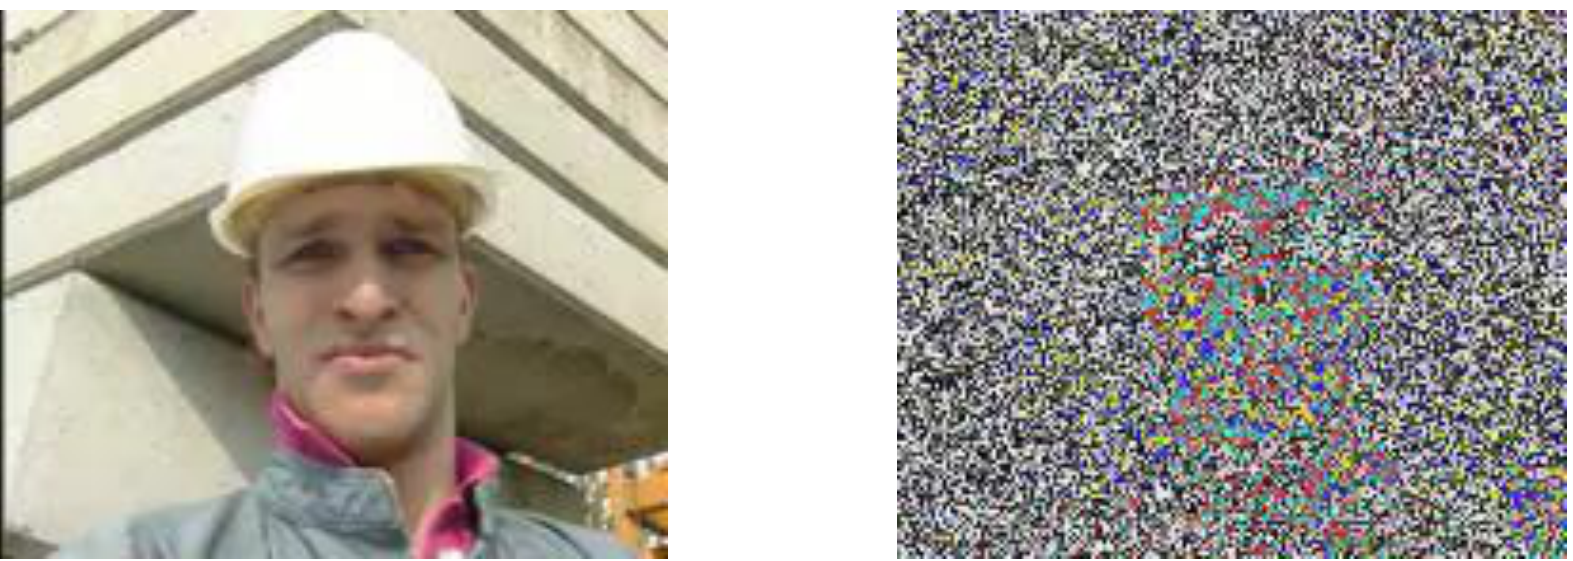
\includegraphics[width=171.99mm,height=154.44mm]{../../images/llm/page_034_img_01.png}%
\end{textblock*}

\end{document}
